\documentclass{article}
\usepackage[utf8]{inputenc}
\usepackage{mathtools}
\usepackage[norsk]{babel}
\usepackage{wrapfig}
\usepackage{fullpage}

\usepackage{listings}
\usepackage{enumitem, hyperref}
\usepackage{graphicx}
\usepackage{tikz}

\usetikzlibrary{trees}
\usepgflibrary{arrows}
\usetikzlibrary{arrows}
\usetikzlibrary{graphs}
%\usetikzlibrary{graphdrawing}
\usetikzlibrary{shapes.geometric,arrows,fit,matrix,positioning}


%\tikzset
%{
%    treenode/.style = {circle, draw=black, align=center, minimum size=1cm},
%    subtree/.style  = {isosceles triangle, draw=black, align=center, minimum height=0.5cm, minimum %width=1cm, shape border rotate=90, anchor=north}
%}




\title{Sammendrag Superdatat}
\author{torholmslettebak }
\date{07.01.2015}

\begin{document}

\maketitle
\tableofcontents
\section{Introduction}

\section{Supercomputing}
Using computers to solve problems which are compute intensive, i.e., problems which require large computing resources in terms of memory or floating point operations or both.
Good examples are weather forecast, oil exploration, seismic analysis and computational mechanics.

Due to the resource demanding aspects of supercomputing, it is important to make the whole solution process as efficient as possible. Several fields are important to study:  numerical/computational algorithms, as fast, robust and accurate as possible, the software development, treatment of large data sets, visualization, and validation of the simulation results.

Supercomputing implies the use of parallel processing, which means underlying algorithms need to be designed and tuned for this environment, to efficiently share information between processor units.  
\subsection{Solution time on supercomputer}
Let $T_{1}$ be the solution time of some problem on a single-processor machine. Assume that we port this simulation to a multi-processor system with P processors. Ideally the solution time would be reduced by a factor of P. We would like a speedup: 
\begin{equation}
S_p = T_{1}/T_{p} = P 
\end{equation}
Where $T_{p}$ is the solution time on P processors. Typically the speedup, $S_{p} < P$. If we increase the number of processors to solve the problem, initially we will have a decent speedup, followed by a degradation as we add more processors. In order to achieve a perfect speedup, we cannot have overhead\footnote{ overhead - combination of excess or indirect computation time, memory, bandwidth, or other resources that are required to attain a particular goal} when moving from single-processor system to a multi-processor system. In reality, we have communication between the processors, i.e. overhead. As the number of processors is increased, the work per processors goes down, while the overall communication (overhead) goes up. One critical issue is therefore to minimize the communication overhead so that we can take advantage of larger systems (at least for fixed problems, more communication needed for unfixed problems). 

\subsubsection{Single-processor performance}
We have to different versions, A and B, of an application. The underlying numerical algorithms are identical. The simulation times denoted as $T_{1}^A$ and $T_{1}^B$. We observe that: 
\begin{equation}
T_{1}^A = 3T_{1}^B
\end{equation}
How can the two simulation times be so different when the numerical algorithms are the same.
\tikzstyle{decision} = [diamond, draw, fill=blue!20, 
    text width=5.0em, text badly centered, node distance=3cm, inner sep=0pt]
\tikzstyle{block} = [rectangle, draw, fill=blue!20,
    text width=6em, text centered, rounded corners, minimum height=4em]
\tikzstyle{line} = [draw, -latex']
\newline
\begin{tikzpicture}[node distance = 3cm, auto]
    \node [block] (init) {Numerical algorithm};
    \node [block, right of=init] (programming) {Programming};
    \node [block, right of=programming] (compiler) {Compiler};
    \node [block, right of=compiler] (executable) {Executable};
    
    \path [line] (init) -- (programming);
    \path [line] (programming) -- (compiler);
    \path [line] (compiler) -- (executable);
\end{tikzpicture}
\newline
A few aspects that can cause this: \begin{itemize}
\item Different choice of data structure / memory layout in programming
\item different use of optimized numerical libraries
\item different choice of compiler optimization
\end{itemize}
Other ways to change solution time for this simulation could be to change the computer, or change the computational/numerical algorithms.

\section{Floating point representation - the IEEE standard}
All real numbers are represented with a finite number of bits. The actual decimal value V of the floating point is: 
\begin{equation}
V = (-1)^S \cdot 2^{E-B} \cdot M
\end{equation}
\begin{figure}[H]
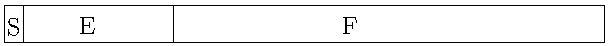
\includegraphics[scale=1.0]{ieee}
\label{floatingpoint}
\caption{Each floating point has a binary representation with three fields: S denotes the sign of the number, E is an exponent, and F is the fraction part of the mantissa}
\end{figure}
A value $S = 0$ means that the number is positive, while S = 1 means that the number is negative. E is an exponent that can be adjusted so that the Mantissa can be expressed as 
\begin{equation}
M = 1 \cdot b_{1} b_{2} ...
\end{equation}


\end{document}
